\documentclass[tikz,border=3.14mm]{standalone}
\usepackage{amsmath}
\usepackage{pgfplots}
\pgfplotsset{compat=1.17}

\begin{document}
    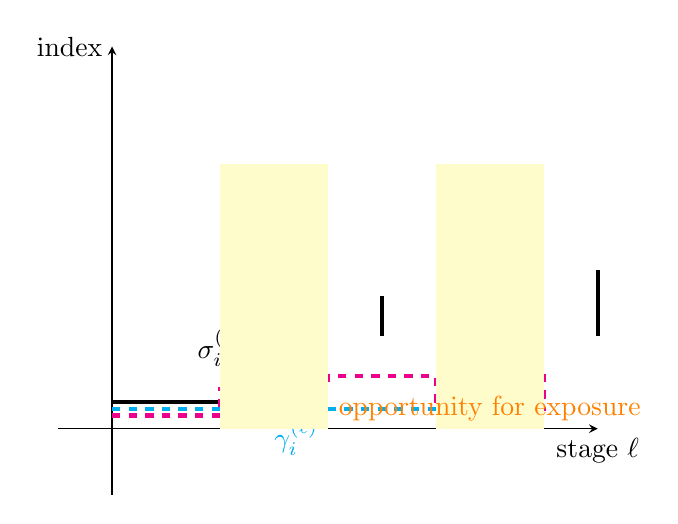
\begin{tikzpicture}
        \begin{axis}[
            axis x line=middle, 
            axis y line=middle,
            xlabel={stage $\ell$}, 
            ylabel={index},
            xlabel style={right, below},
            ylabel style={above, left},
            xtick=\empty,
            ytick=\empty,
            xmin=-0.5,
            xmax=4.5,
            ymin=-0.5,
            ymax=2.5,
            enlarge y limits={rel=0.13, upper},
            clip=false
        ]
            % sigma_i^(l) plot
            \addplot+[
                ycomb,
                mark=none,
                color=black,
                line width=1.5pt,
                domain=1:4,
                samples at={1,...,4},
                shift={(axis cs:0,0.2)}
            ] {0.2+0.1*(x-1)};
            \addplot+[
                mark=none,
                color=black,
                line width=1.5pt,
                domain=0:1,
                samples at={0,1},
            ] coordinates {(0,0.2) (1,0.2)};
            
            % kappa_i^(l) plot (dashed magenta)
            \addplot+[
                mark=none,
                dashed,
                color=magenta,
                line width=1.5pt,
                domain=0:4,
                samples at={0,...,4},
                const plot
            ] coordinates {(0,0.1) (1,0.3) (2,0.4) (3,0.15) (4,0.45)};
            
            % gamma_i^(l) plot (dashed cyan)
            \addplot+[
                mark=none,
                dashed,
                color=cyan,
                line width=1.5pt,
                domain=0:4,
                samples at={0,...,4},
                const plot
            ] coordinates {(0,0.15) (1,0.15) (2,0.15) (3,0.15) (4,0.15)};
            
            % sigma_i^(l) labels
            \node[above] at (1,0.4) {$\sigma_i^{(\ell)}$};
            
            % kappa_i^(l) labels
            \node[below left, magenta] at (2,0.4) {$\kappa_i^{(\ell)}$};
            
            % gamma_i^(l) labels
            \node[below left, cyan] at (2,0.15) {$\gamma_i^{(\ell)}$};
            
            % Highlighted regions (opportunities for exposure)
            \fill[yellow!20] (1,0) rectangle (2,2);
            \fill[yellow!20] (3,0) rectangle (4,2);
            \node[orange] at (3.5,0.15) {opportunity for exposure};
        \end{axis}
    \end{tikzpicture}
\end{document}